% $Id$
% vim: tw=78 ai spell spelllang=en

\documentclass[10pt]{llncs}
\usepackage{color}
\usepackage{url}
\usepackage{xspace}
\usepackage{graphicx}
\usepackage{listings}

%{{{ LaTeX definitions

\newcommand\Color[2]{\textcolor{#1}{#2}}
\newcommand{\nb}[1]{\marginpar{\scriptsize #1}}
\renewcommand\note[1]{\nb{\Color{blue}{#1}}}
\newcommand\todo[1]{\nb{\Color{red}{#1}}}

\newcommand{\Stanse}{\textsc{Stanse}\xspace}
\newcommand{\TC}{\textsc{ThreadChecker}\xspace}
\newcommand{\AC}{\textsc{AutomatonChecker}\xspace}
\newcommand{\RC}{\textsc{ReachabilityChecker}\xspace}

\lstset{tabsize=2,numbers=none,showstringspaces=false,breaklines=true,
        breakatwhitespace=true,escapeinside={(*@}{@*)},
	basicstyle=\scriptsize}

%}}}

\begin{document}

%{{{ Title+Authors+Abstract

\title{{STANSE}: Bug-finding Framework\\ for C Programs}
\author{Jan~Obdr\v{z}\'alek, Ji\v{r}\'\i~Slab\'y, Jan Strej\v{c}ek and Marek~Trt\'{\i}k}
\institute{Faculty of Informatics, Masaryk University, Brno, Czech Republic\\
\email{\{obdrzalek,slaby,xstrejc,trtik\}@fi.muni.cz}}

\maketitle

\begin{abstract}
\Stanse is a modular framework, available free under the GPLv2 license, for finding bugs in C programs using static analysis. Its two main design goals are applicability on large software projects like Linux kernel and extensibility with new bug-finding techniques with a minimal effort. There are currently three bug-finding algorithms implemented within \Stanse: \AC checks properties described in an automata-based formalism, \TC detects deadlocks among multiple threads, and \RC looks for unreachable code. \Stanse has been tested on the Linux kernel, where it has found dozens of previously undiscovered bugs.
\end{abstract}

%}}}

%{{{ Intro

\section{Introduction}
\label{sec:introduction}

Bug-finding based on static analysis have finally come of age in the last decade. One of the papers to really stir interest was~\cite{ECCH00}, showing that static analysis can efficiently find many interesting bugs in a real-world code, as demonstrated on the Linux kernel. This work eventually led to a successful commercial tool called \textsc{Coverity}~\cite{coverity}. Over the years, several other successful tools, like \textsc{CodeSonar}~\cite{codesonar}\todo{Unmatched citation} or \textsc{Klocwork}~\cite{klocwork}, appeared.

However, such fully-featured tools are neither free to obtain, nor is their code available (e.g.~for developing new algorithms or tailoring the existing tools to specific tasks). The existing free tools are usually severally limited in what they can do (e.g.~\textsc{Uno}~\cite{uno}, \textsc{Sparse}~\cite{sparse}, \textsc{Smatch}\todo{Missing citation}). One notable exception is \textsc{FindBugs}~\cite{HP04,findbugs}, a successful tool working on Java code.

\Stanse is intended to fill this gap for C language. \Stanse can be viewed in following two general ways:
\begin{enumerate}
\item \Stanse \emph{framework}: a robust Java library for implementing diverse static analysis algorithms. An implemented algorithm can be immediately evaluated on large real-world software projects written in C as the framework is capable to process such projects. For example, it can process the whole Linux kernel. An implementation of such an algorithm within the framework is called \emph{checker}.
\item \Stanse \emph{tool}: a Java application, which integrates \Stanse framework and provides a user user friendly way, how to apply the framework. It comprise command line options, GUI, and tracing error reports.
\end{enumerate}

%The rest of the paper is structured as follows. Section~\ref{sec:framework} describes the functionality provided by the framework, while Section~\ref{sec:checkers} is devoted to the three existing checkers. Section~\ref{sec:results} presents some results of \Stanse evaluation on the Linux kernel. The last section summarizes the basic strengths of \Stanse and mentions some directions of its future development.

\section{Tool Usage}

Here we describe an usage of tool \Stanse. We focus at a pipeline an user typically follows to analyse a source code. Each subsection describes one step of the pipeline.

\subsection{Selecting Source Files}

There are several ways to tell \Stanse what source files to analyse. Besides the standard possibilities, comprising a single given file, all files from a given directory, all files listed in a given file, \Stanse can also derive all the necessary information from a project \textsf{Makefile}. In the C language family case \todo{Why is there: "In the C language family case"}, it also remembers compiler flags for preprocessing purposes. This functionality was inspired by the \textsc{Sparse}~\cite{sparse} tool. \Stanse can currently process source files written in C language fulfilling the ISO/ANSI C99 standard and possibly including almost all of the GNU C extensions.

\subsection{Specifying checkers}

A static analysis algorithm integrated into \Stanse is called a \emph{checker}. An user can choose, which checkers should be applied to selected source files. This is very simple procedure for the user, since it only consists of choosing appropriate checkers from a list of checkers, plus choose for each checker, whether interprocedural or intraprocedural variant of a checker should be used.

\subsection{Executing checkers}

When an user is done specifying source files and checkers to be applied, the verification can start. For an user it means to \emph{push a button}. The verification is then completely autonomous, it does not require any user's assistance. The user can just watch the progress of the execution in the output window. When the execution is finished, a complete list of \emph{error reports}, found by checkers, is showed to the user.

\subsection{Processing Error Reports}

An error report represent a path in the source code leading to an error. For each source code line along the path of the report there is an information attached explaining what is going on at the line. Tool \Stanse provides several possibilities to present the error reports: they can be printed to the console, displayed using a built-in GUI browser, or saved to an external file. In the GUI browser an user can trace each report per line of the source files and read the attached information. Since some of the reports may be false alarms, the user can mark reports in the browser as real errors or false alarm to distinguish them. The browser window is shown in Figure~\ref{fig:bugreport}.

\todo{There are not marked errors and false alarms in the Figure~\ref{fig:bugreport}!}
\begin{figure}[t]
  \centering
    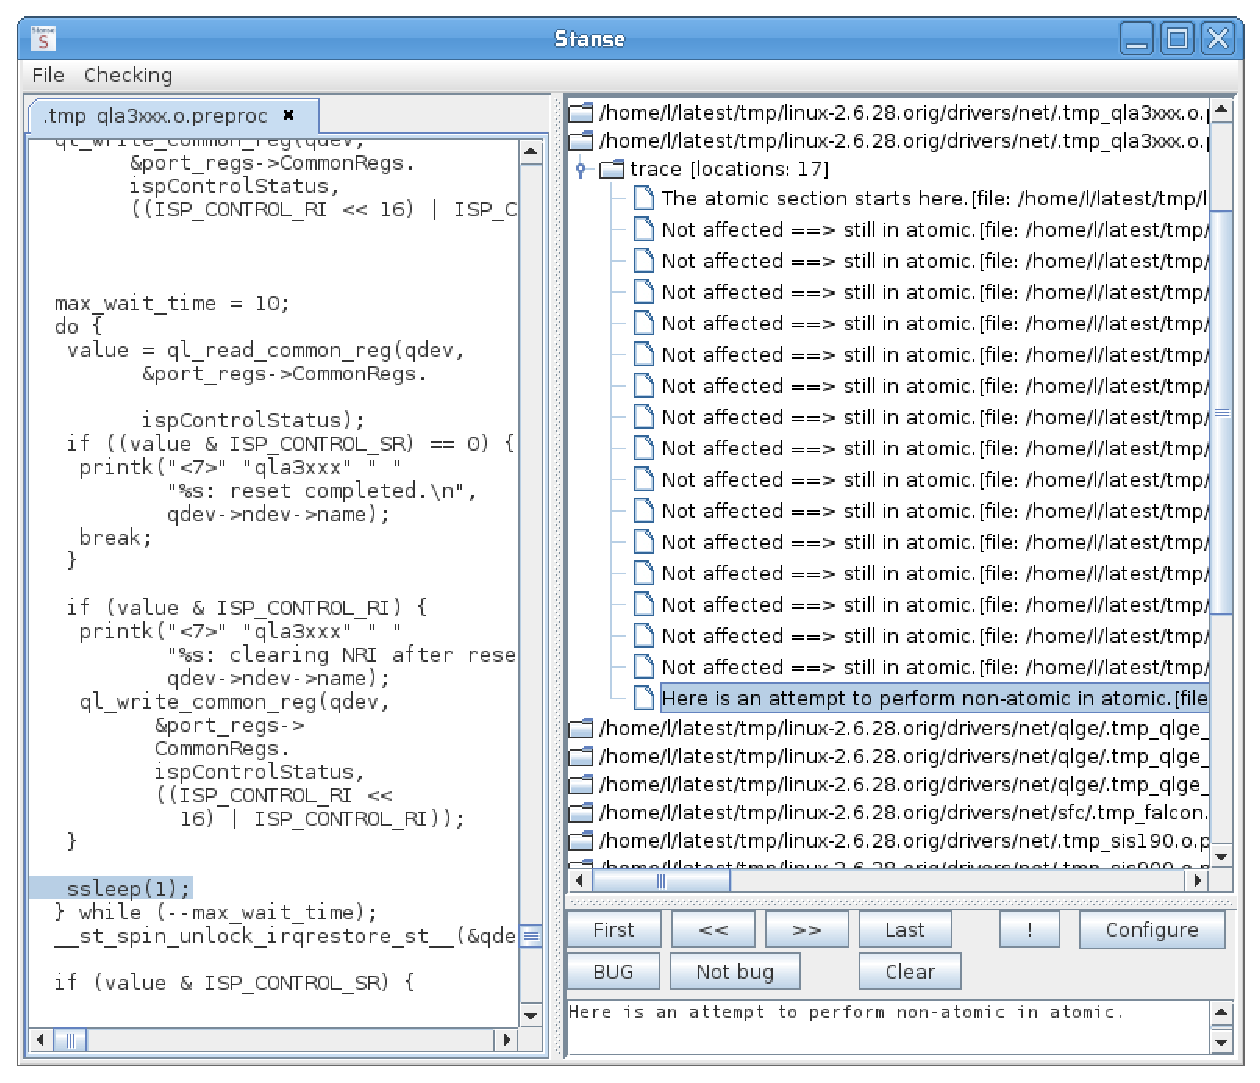
\includegraphics[width=10cm]{screen-bug-tracing}
  \caption{The GUI browser of error reports.}
  \label{fig:bugreport}
\end{figure}

\section{\Stanse Framework}
\label{sec:framework}

\Stanse framework is a Java library which is responsible for verification itself. When the framework is passed filled \emph{Configuration}, which means list of source files and list of checkers to be applied, it handles files parsing and executing checkers and collecting error reports. The list of error report is an output from the library. In the following we describe main concepts and properties of the framework's functionality.

\subsection{Concept of Checkers}

A \emph{checker} is an implementation of a static analysis technique. There can be many checkers simultaneously running in \Stanse, but they do not see each other. They run independently. The checkers share read-only lazy representation of checked program and they are gained an access to the libraries providing common types of navigation in a code.

The checkers are integrated to the framework of \Stanse using concrete factory design pattern. So to insert a new checker to the framework of \Stanse one only needs to (a) implement general checker interface, and (b) register the checker
to the checkers' factory of the framework. Then the checker has full access to the features of the \Stanse and is immediately ready for checking large software projects, like Linux kernel.

\subsection{LazyInternalStructures}

The code to be verified is parsed into set of ASTs, CFGs, and call-graphs, representing \emph{internal structures}. These structures can be accessed by checkers through common interface called \emph{LazyInternalStructures}. Since the interface provides only read access, the checkers share the internal structures. Checkers may attach their data to internal structures using for example hash tables, etc. In addition, the interface provides interprocedural or intraprocedural access  to the internal structures, depending on the variant of the checker.

There is another important property of the interface LazyInternalStructures. Besides providing common access to internal structures it also enables \emph{streaming}.

\subsection{Streaming}

As mentioned earlier, the design of the framework focus at large software projects. Such projects consist of hundreds or
thousands of modules (compilation units). In practice, it is often impossible to store all the corresponding internal structures in the memory. The \Stanse framework therefore applies automatic \emph{streaming} of the internal structures, currently on a module basis.

Instead of parsing all source modules at the beginning, a module is streamed in only when \Stanse needs to access some internal structures corresponding to the module. In other words, the internal structures are constructed in a lazy manner -- we call them \emph{lazy internals}. If the memory occupied by internal structures exceeds a given limit, some internal structures have to be freed before another module is streamed in. The implemented least-recently-used algorithm discards the structures of a module if they are not accessed for a significant time. If the discarded structure is later accessed again, the corresponding module is streamed back in. The streaming is completely transparent to checkers. It means that checkers may assume all the modules are loaded in the memory all the time. It is framework's responsibility to optimally plan streaming of modules in the memory to provide checkers the illusion that all the modules are in the memory.

\subsection{Traversing the Parsed Code}
\label{sec:traverse}

Although all the internal structures are ready to be fully used by a checker at this point, the checker would have to walk through the structures on its own. To prevent unnecessary reimplementations, the most important and heavily used traversal methods are implemented directly inside the framework. A checker can simply use this functionality by specifying
\begin{itemize}
\item whether it should go through the structures forwards or backwards, breath-first or depth-first,
\item if the interprocedural walk-through should be performed or not, and
\item derive a visitor object whose callback method \texttt{visit()} will be called for each visited node in CFG.
\end{itemize}

\subsection{Statistics of Error Reports}

One may need to know some statistical information about error reports obtained from the verification. The framework contains library, which provides such computations. An user may compute information like how many error reports were received from a source file, how many percent of reports were generated from a specific checker, percentage of some type of error report to all reports, how many reports were already sorted to real errors and false alarms, etc.

\subsection{Quick IDE integration}

Since the framework is just Java library, it immediately gives the developers an opportunity to reuse the \Stanse framework for quickly implement plug-in for some IDE.

\section{Checkers}
\label{sec:checkers}

In this section we describe the three currently available checkers.

\subsection{\AC}

This checker is heavily influenced by \cite{ECCH00}. It takes, as an input, a set of finite-state automata, which describe some property which we want to check. Properties like locking discipline, interrupt management, null pointer dereference, dangling pointers and many others can be handled this way.

Compared to the implementation described in~\cite{ECCH00} and \cite{HCXE02}, the technique used  differs in several aspects. Here is a list of the most important differences: (1) we do not use metacompilation, (2) automata are not input-language specific, (3) the interprocedural analysis is done within a single compilation unit.

\subsection{\TC}

\TC aims to check for possible deadlocks in concurrent programs. The technique used is based on the notions of locksets of~\cite{relay} and deadlock detection by looking for cycles in resource allocation graphs (RAG). \TC first tries to identify the parts of the code which can run in parallel, as different threads. Then it builds a set of \emph{dependence graphs} for each such thread. A dependence graph statically represents the possible locksets during one execution of a thread. Dependency graphs are then combined and all cycles examined, by building the corresponding RAGs.

\subsection{\RC}

\RC searches the internals, a CFG more concretely, for unreachable nodes. These are then reported as warnings or errors, depending on importance (e.g. superfluous semicolons are less important than unused branch). This is an easy task and so the writing of such code should be. The code of the checker is below 200 lines including importance decision and much of strings and comments. So it tries to fully demonstrate the power of the \Stanse framework and its primary goal is exactly that. The tool is thus very easy to extend, the checker implementers can focus on real techniques.

%}}}
%{{{ Results

\section{Results -- Linux Kernel}
\label{sec:results}

We are exercising the Linux kernel by \Stanse since 2.6.28 was released back
in 2008. It was the first release we decided to test the usability of \Stanse
on. One reason to choose the Linux kernel is that it represents a large and
freely available codebase, where the absence of bugs is of great concern.
Moreover, the Linux kernel fully exercises most features of ANSI C99 and GNU C
extensions. The other motivation is to provide a free tool for Linux kernel
developers.

Currently, \textsc{Coverity Prevent}~\cite{coverity} is daily run on the
current development branch of the Linux kernel, and the results are reported
back to developers. However, developers kept asking for a tool with which
their code will be checked before it appears upstream. Moreover, the kernel
code is very specific and the tool should consider these specifics.

We used all three checkers described above. These checkers are not kernel
specific and only the configuration for \AC has to be tailor-made to look for
the type of bugs commonly found in the kernel code. The properties checked by
the \AC in the kernel are:
\begin{itemize}
\item correct pairing of functions like balanced locking, check for correct
  reference counting,
\item memory/pointer related bugs like dereferencing null pointers and
\item atomic section restrictions to find if someone can cause deadlocks by
sleeping inside spinlocks or interrupt handlers.
\end{itemize}

\begin{figure}[tb]
\begin{center}
\begin{tabular}{c}
\begin{lstlisting}[language=C]
static void untag_chunk(struct node *p) {
 spin_lock(&entry->lock);
 ...
 new = alloc_chunk(size);
 ...
 spin_unlock(&entry->lock);
}
static struct audit_chunk *alloc_chunk(int count) {
 ...
 chunk = kzalloc(size, GFP_KERNEL);
\end{lstlisting}
\end{tabular}
\end{center}
\caption{Bug found in the audit code}
\label{fig:error}
\end{figure}

With this configuration, the running time of \Stanse on a common desktop
machine with 2 cores and 4\,GiB of memory is under 100 minutes. With
streaming, the memory usage of the Java process oscillates between 400 and
1000\,MiB in case of forced garbage collector executions. The standard \Stanse
\textsf{Makefile} support was used and we did not have to manually tweak the
source code in any way in order to be processed by \Stanse.

In the 2.6.28 release, more than 70 bugs\footnote{A list of confirmed bugs is
available at \url{http://stanse.fi.muni.cz/bugs.html}} were reported to kernel
developers, most with appropriate patches, and fixed in the next kernel
release. Some of these bugs remained undiscovered for seven
years\footnote{\url{http://lkml.org/lkml/2009/3/11/380}}. This is despite the
kernel being daily
checked\footnote{\url{http://marc.info/?l=linux-kernel&m=125856033627134&w=2}}
with \textsc{Coverity Prevent} and we believe it is due to the filters they
use.

Now we present one bug which we found in the code reporting security
incidents. An excerpt from the particular code is in the
Figure~\ref{fig:error}.  \texttt{untag\_chunk} functions creates a critical
section by a spinlock and calls \texttt{alloc\_chunk} which in turn can sleep
in \texttt{kzalloc}. This can, under certain circumstances, lead to deadlock
of the whole system. The bug was confirmed and fixed.

The false positive (FP) rate oscillates among the different bug types, the
overall ratio is that 40\,\% of all reported errors are real bugs. This result
is quite low, however similarly to~\cite{havoc}, it is without any thorough
false-positive filtering techniques (cf. Future Work section). The more
detailed results about the \AC are in the Table~\ref{tab:results}, one row
per each configuration.

\begin{table}[tb]
\begin{center}
\begin{tabular}{|l|r|r|r|r|r|} \hline
\textbf{Automaton} & \textbf{Errors} & \textbf{Assorted} & \textbf{Bugs} &
\textbf{FP} & \textbf{Ratio} \\ \hline\hline
\textit{Pairing} & 266 & 58 & 65  & 143 & 31.3\,\% \\ \hline
\textit{Memory}  & 86  & 1  & 48  & 37  & 56.5\,\% \\ \hline
\textit{Atomic}  & 35  & 1  & 16  & 18  & 47.1\,\% \\ \hline\hline
\textbf{Overall} & 387 & 60 & 129 & 198 & 39.4\,\% \\ \hline
\end{tabular}
\end{center}
\caption{Errors found by \AC in the 2.6.28 Linux kernel. Assorted = Neroztrizene = nepodarilo se rozhodnout.}
\label{tab:results}
\end{table}

The current kernel versions are checked with other tools like
\textsc{Coccinelle} or \textsc{Smatch}. Mostly these tools find simple pattern
matching style properties like lock-unlock and are successful at that. We
continue to check the kernel releases with \Stanse too and, thanks to
interprocedural analysis, we still are able to find errors on daily basis.

The most convenient advantage on these tools is their availability. The
developers or testers can take them whenever they want and check their code
instantly, because they are freely available and they can handle the kernel
code. Further these tools need near no configuration (either because they
provide predefined one or there is nothing to configure) and are ready to use
out of the box.

%}}}
%{{{ Conclusion

\section{Conclusion}

%\subsection{Future Work}
%C++ support, rewrite to C, get rid of XML, daily analysis, results difference.
%Should this be here? Pay attention, we reference future work section above.
%
%\subsubsection{Parser:} ... but the parser itself is
%generated by \textsc{ANTLR} from a top-down C grammar which we developed
%based on provided example grammar. This is a limiting factor of the whole
%tool when parsing C sources, because (according to the \textsc{ANTLR}
%authors) the C parser in Java is unoptimized and slow -- this is not true
%for C parser in C, so we use it for parsing included headers to extract type
%definitions. The rest of file is handled in Java.
%
%Nowadays, we are working hard on merging a C++ support which is based on
%\textsc{clang++} from \textsc{LLVM} suite and we are almost finished. We do
%not use \textsc{clang} (at the time of writing this article, 2.8 is stable)
%for pure C because it still misses some features from the GNU C which are
%widely used in the Linux kernel (at least local labels and some assembler
%constraints explicitly).
%
%interni struktury jsou popsany v XML a to je spatne.
%
%There is a plan to integrate \Stanse at least into \textsc{Eclipse}.

\subsubsection{Acknowledgements}
\label{sec:acknowledgements}

Jan Ku\v{c}era is the author of the \TC. We would like to thank Linux kernel
developers, and Cyrill Gorcunov for \Stanse alpha testing and useful
suggestions. All authors are supported by the research centre Institute for
Theoretical Computer Science (ITI), project No. 1M0545.

%}}}

\bibliographystyle{plain}
\bibliography{stanse}

\end{document}

\section{What's Missing}
There are several points we miss which were commented in the past reviews.
They include:
\begin{itemize}
\item soundness, completeness
\item scalability, applicability
\item full bugs description
\end{itemize}

Markovo summary:
\begin{itemize}
\item �e jde v prvn� �ad� o framework pro statickou anal�zu. Tedy �e
  nab�z�me funk�n� bal�k k�du, do kter�ho se d� s minim�ln�m �sil�m
  naimplementovat jist� konkr�tn� nov� technika.
\item Co tedy framework nab�z�: Configuration,
  LazyInternals(ASTs,CFGs,Streaming), Inter/Intra-anal�zy, Traversov�n�,
  Statistics, GUI.
\item Pro otestov�n� frameworku m�me naps�no n�kolik checker�
  (Automaton,...). \Stanse jsme byli schopni pustit na cel� kernel Linuxu a
  nal�zt v n�m n�kolik chyb.
\end{itemize}

%%% Local Variables:
%%% mode: latex
%%% TeX-command-default: "LaTeX"
%%% End:
